\documentclass[11pt,a4paper]{article}
\usepackage[utf8]{inputenc}
\usepackage[T1]{fontenc}
\usepackage{lmodern}
\usepackage[a4paper,margin=2.2cm]{geometry}
\usepackage{setspace}\onehalfspacing
\setlength{\parskip}{0.4em}\setlength{\parindent}{1.2em}
\usepackage{amsmath,amssymb}
\usepackage{booktabs,tabularx,array}
\renewcommand{\arraystretch}{1.2}
\usepackage{graphicx}
\usepackage[shortlabels]{enumitem}
\usepackage{fancyhdr}
\pagestyle{fancy}\fancyhf{}
\fancyhead[L]{\small\textsc{Mineração de Séries Temporais} -- Atividade da Aula 2}
\fancyhead[R]{\small\thepage}
\renewcommand{\headrulewidth}{0.4pt}
\usepackage[hidelinks]{hyperref}
\usepackage[most]{tcolorbox}
\newtcolorbox{resposta}[1][]{enhanced,breakable,colback=white,colframe=black,boxrule=0.5pt,leftrule=3pt,arc=0pt,outer arc=0pt,fonttitle=\bfseries\small,title=Resposta,#1}
\usepackage{listings}
\lstset{language=Python,basicstyle=\ttfamily\footnotesize,keywordstyle=\bfseries,commentstyle=\itshape,showstringspaces=false,breaklines=true,frame=single,framerule=0.3pt,columns=fullflexible,keepspaces=true,
literate={á}{{\'a}}1 {ã}{{\~a}}1 {é}{{\'e}}1 {ê}{{\^e}}1 {í}{{\'i}}1 {ó}{{\'o}}1 {õ}{{\~o}}1 {ú}{{\'u}}1 {ç}{{\c{c}}}1}
\renewcommand{\figurename}{Figura}\renewcommand{\tablename}{Tabela}

\title{\bfseries Atividade da Aula 2 -- Forecasting da série UNRATE com ETS e LSTM}
\author{César Willian Pacheco\\ \small Especialização em Inteligência Artificial \& Ciência de Dados -- PUCPR\\ \small Prof.\ Vinícius Mourão Alves de Souza}
\date{Setembro de 2026}

\begin{document}
\maketitle
\thispagestyle{fancy}

\section*{Enunciado e dados}
Dada a série UNRATE (taxa mensal de desemprego nos EUA desde 1948): fazer as previsões das últimas 12 observações com o modelo ETS e com o modelo LSTM e responder qual modelo apresentou o menor erro (RMSE).

A série foi obtida diretamente do FRED (\url{https://fred.stlouisfed.org/series/UNRATE}), a mesma fonte do arquivo \texttt{UNRATE.csv} do professor: 944 observações mensais de janeiro/1948 a agosto/2026, taxa \emph{dessazonalizada} (\textit{seasonally adjusted}) pelo BLS. A observação de outubro/2025 não foi publicada (paralisação do governo americano) e aparece como ``.'' no arquivo; ela foi removida com \texttt{dropna()}, a mesma convenção do notebook do professor, restando 943 valores. Todos os resultados foram gerados pelo script \texttt{forecasting\_unrate.py} (statsmodels 0.15, TensorFlow/Keras 2.21), anexo.

\section{Protocolo experimental}
\begin{itemize}[leftmargin=*]
\item \textbf{Holdout temporal.} Teste = as \textbf{12 últimas observações} (agosto/2025 a agosto/2026, sem outubro/2025); treino = as 931 anteriores. Nada é embaralhado: a validação cruzada aleatória vazaria informação do futuro para o passado.
\item \textbf{Métrica.} $\text{RMSE} = \sqrt{\tfrac{1}{12}\sum (y_i - \hat y_i)^2}$, em pontos percentuais de desemprego; MAE e MAPE são reportados como apoio.
\item \textbf{Baselines.} Mean, naive (repete o último valor) e drift, como referência da dificuldade do problema.
\item \textbf{Sem vazamento.} A escolha da configuração do ETS usa o AICc calculado \emph{no treino}; a escolha da configuração da LSTM usa a perda de \emph{validação} (últimos 20\% das janelas de treino); o \texttt{MinMaxScaler} é ajustado só no treino. O conjunto de teste é usado uma única vez, ao final.
\end{itemize}

\begin{figure}[h]\centering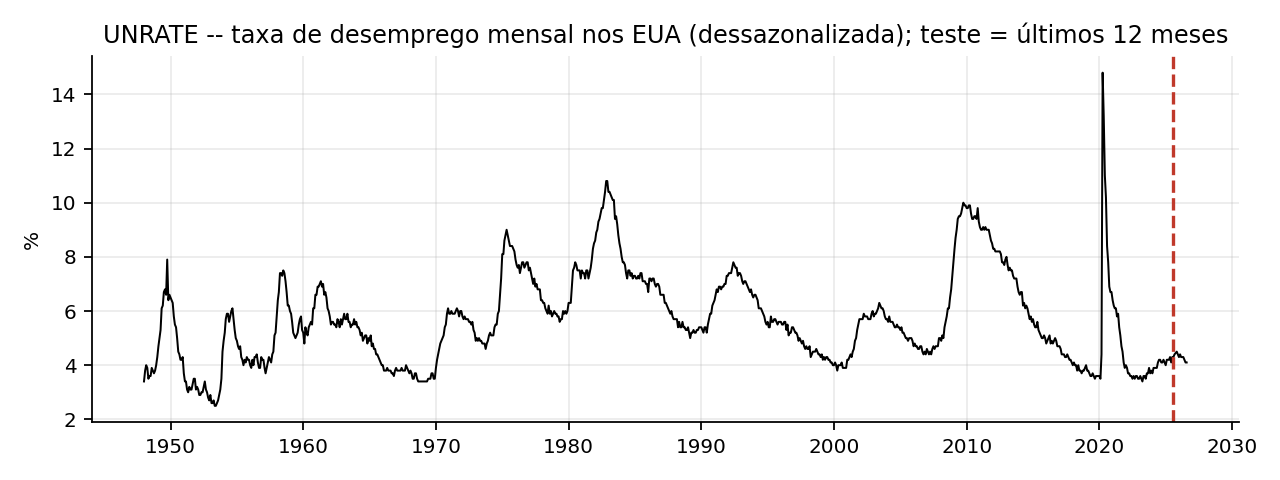
\includegraphics[width=0.95\linewidth]{figuras/serie.png}
\caption{UNRATE (1948--2026). A linha tracejada marca o início das 12 observações de teste.}\end{figure}

\section{ETS: escolha da configuração e resultado}
\begin{resposta}
\textbf{Justificativa da configuração.} A série tem \emph{nível} que muda lentamente e \emph{ciclos} de duração irregular (recessões e expansões, como mostrado na Aula 1), mas \textbf{não tem sazonalidade} -- ela já é publicada dessazonalizada -- e não tem uma tendência global (oscila entre 2,5\% e 14,8\% e termina próximo de onde começou). Logo, os candidatos naturais são os modelos \emph{sem componente sazonal}: ETS(A,N,N) (só nível, equivalente à suavização exponencial simples), ETS(A,A,N) (Holt, com tendência aditiva) e ETS(A,Ad,N) (tendência amortecida). Versões com sazonalidade aditiva ($m=12$) foram ajustadas apenas para confirmar que não ajudam. O erro é aditivo porque a amplitude das flutuações não cresce com o nível da série. A seleção entre candidatos foi feita pelo \textbf{AICc no treino} (Hyndman \& Athanasopoulos, cap.~8), sem olhar o teste.
\end{resposta}

\begin{center}\small
\begin{tabular}{@{}lrrrr@{}}
\toprule
\textbf{Modelo} & \textbf{Parâmetros} & \textbf{AICc (treino)} & \textbf{RMSE (teste)} & \textbf{MAE (teste)} \\
\midrule
\textbf{ETS(A,N,N)} & 2 & \textbf{1010,44} & \textbf{0,1155} & 0,0833 \\
ETS(A,A,N) & 4 & 1014,57 & 0,1183 & 0,0872 \\
ETS(A,Ad,N) & 5 & 1015,58 & 0,1155 & 0,0834 \\
ETS(A,N,A), $m=12$ & 15 & 1027,29 & 0,1533 & 0,1368 \\
ETS(A,A,A), $m=12$ & 17 & 1031,53 & 0,1546 & 0,1372 \\
ETS(A,Ad,A), $m=12$ & 18 & 1032,69 & 0,1525 & 0,1358 \\
\midrule
Baseline mean & -- & -- & 1,3768 & 1,3720 \\
Baseline naive & -- & -- & 0,1155 & 0,0833 \\
Baseline drift & -- & -- & 0,1183 & 0,0872 \\
\bottomrule
\end{tabular}
\end{center}

\begin{resposta}[title={Resultado do ETS}]
O modelo selecionado é o \textbf{ETS(A,N,N)}, com $\alpha = 0{,}9999$ e nível inicial 3,40. Com $\alpha \approx 1$ a equação do nível $\ell_t = \alpha x_t + (1-\alpha)\ell_{t-1}$ reduz-se a $\ell_t = x_t$: a previsão para todo o horizonte é o último valor observado, $\hat y_{t+h} = 4{,}3$ para $h = 1,\dots,12$. Ou seja, o melhor ETS \textbf{coincide com o baseline naive}, e a tabela mostra que tendência (Holt) e sazonalidade só pioram o AICc e o erro de teste. Isso não é uma falha do método: a taxa de desemprego mensal comporta-se como um passeio aleatório -- mudanças pequenas e persistentes, sem padrão sazonal --, e para esse tipo de série a teoria diz que a melhor previsão pontual é o valor corrente. \textbf{RMSE do ETS = 0,1155} pontos percentuais (MAE 0,083; MAPE 1,95\%).
\end{resposta}

\section{LSTM: arquitetura, hiperparâmetros e resultado}
\begin{resposta}
\textbf{Arquitetura (deliberadamente pequena).} Segue o notebook do professor: entrada com $w$ passos e 1 variável $\rightarrow$ camada \texttt{LSTM(u)} $\rightarrow$ camada \texttt{Dense(12)} que emite os 12 valores de uma vez (abordagem \emph{direta}, multi-output, que evita o acúmulo de erros da abordagem recursiva). Otimizador Adam, perda MSE, \textit{batch} 8, até 300 épocas com \textit{early stopping} (paciência 20, restaurando os melhores pesos) monitorando os últimos 20\% das janelas de treino (\texttt{shuffle=False}, para que a validação seja o trecho mais recente). A série é escalada para $[0,1]$ com \texttt{MinMaxScaler} ajustado só no treino.

\textbf{Seleção da janela e das unidades.} Testaram-se $(w,u) \in \{(12,8), (24,8), (24,16), (36,8)\}$, escolhendo pela perda de validação média de 3 sementes:
\begin{center}\small
\begin{tabular}{@{}cccrr@{}}
\toprule
$w$ & $u$ & janelas de treino & parâmetros & perda de validação (MSE, escala [0,1]) \\
\midrule
\textbf{12} & \textbf{8} & 908 & 428 & \textbf{0,01522} \\
24 & 8 & 896 & 428 & 0,01566 \\
24 & 16 & 896 & 1356 & 0,01550 \\
36 & 8 & 884 & 428 & 0,01617 \\
\bottomrule
\end{tabular}
\end{center}
A configuração final tem \textbf{janela de 12 meses, 8 unidades LSTM e 428 parâmetros treináveis}; o treinamento parou entre 37 e 51 épocas. Como os pesos iniciais são aleatórios, o modelo foi treinado com 5 sementes (0 a 4).
\end{resposta}

\begin{center}\small
\begin{tabular}{@{}lrrr@{}}
\toprule
\textbf{Execução da LSTM} ($w=12$, $u=8$) & \textbf{RMSE} & \textbf{MAE} & \textbf{épocas} \\
\midrule
semente 0 (execução principal) & 0,3720 & 0,3058 & 41 \\
semente 1 & 0,3981 & 0,3003 & 51 \\
semente 2 & 0,3768 & 0,2933 & 42 \\
semente 3 & 0,3633 & 0,2700 & 37 \\
semente 4 & 0,3452 & 0,2666 & 39 \\
\midrule
média $\pm$ desvio das 5 sementes & 0,3711 $\pm$ 0,0173 & & \\
previsão média das 5 sementes (\textit{ensemble}) & 0,3643 & & \\
\bottomrule
\end{tabular}
\end{center}

\begin{figure}[h]\centering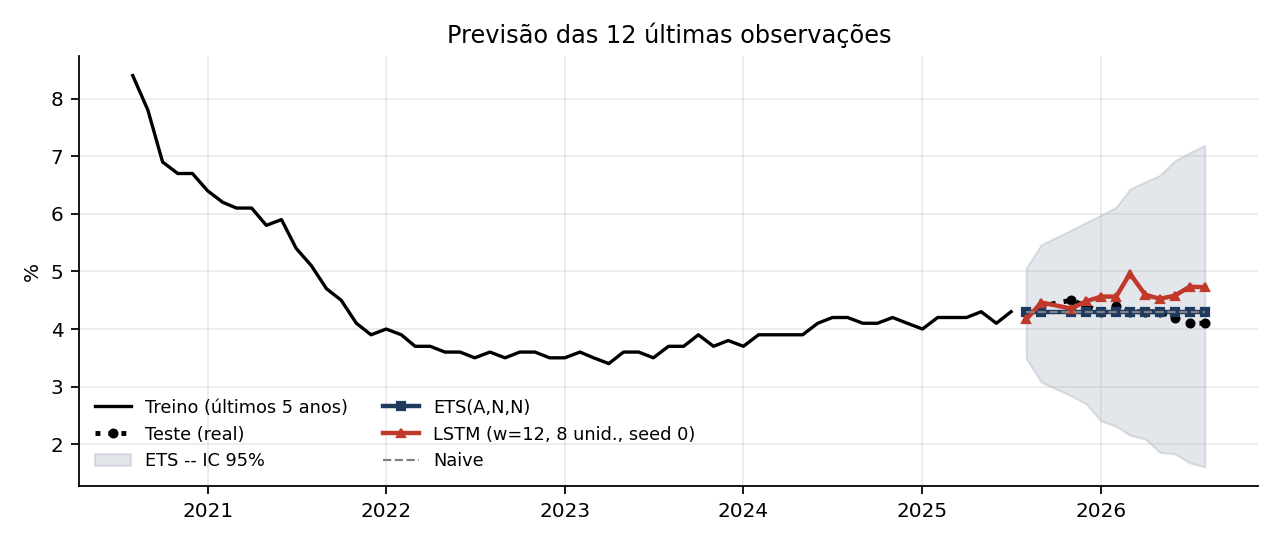
\includegraphics[width=0.95\linewidth]{figuras/previsoes.png}
\caption{Últimos cinco anos de treino, valores reais de teste e previsões do ETS(A,N,N) (com intervalo de 95\% simulado) e da LSTM.}\end{figure}

\begin{figure}[h]\centering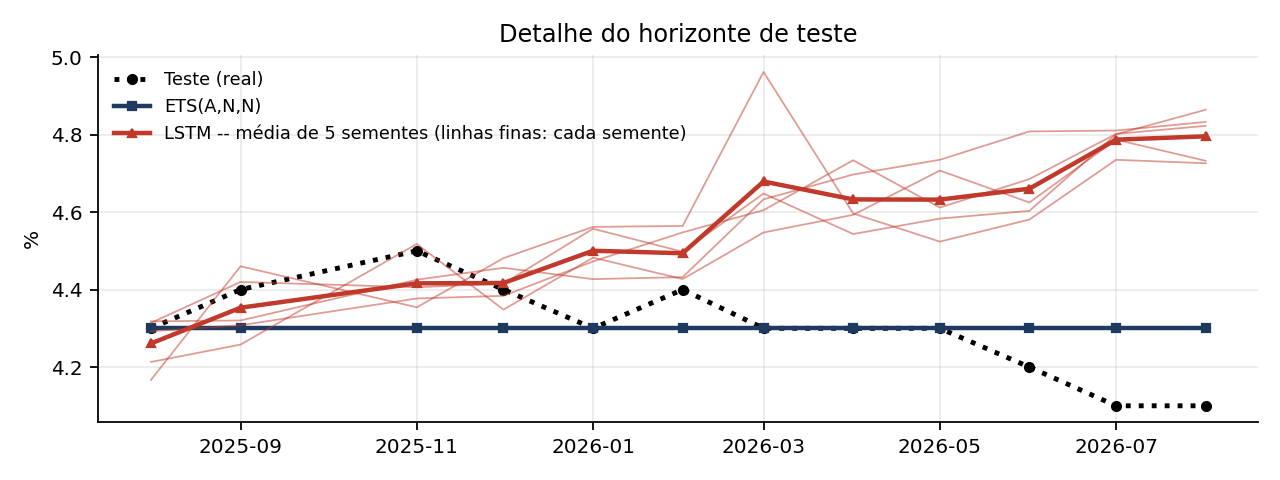
\includegraphics[width=0.95\linewidth]{figuras/detalhe.png}
\caption{Detalhe do horizonte de teste: cada linha fina é uma semente da LSTM; a linha grossa é a média.}\end{figure}

\section{Qual modelo apresentou o menor RMSE -- e por quê}
\begin{resposta}
\textbf{O ETS venceu com folga: RMSE = 0,116 contra 0,371 $\pm$ 0,017 da LSTM (3,2 vezes maior).} Nenhuma das cinco sementes da LSTM (melhor caso 0,345) chegou perto do ETS, e nem a média das cinco previsões (0,364). A LSTM previu uma \emph{alta} gradual do desemprego, de 4,3\% para $\approx 4{,}8\%$, enquanto a série ficou estável e depois caiu para 4,1\%; o ETS previu simplesmente 4,3\% e errou, em média, 0,08 ponto.

\textbf{Por que isso acontece} (relacionando com o que foi visto em aula):
\begin{enumerate}[leftmargin=*]
\item \textbf{Natureza da série.} A UNRATE é dessazonalizada, sem tendência global e com autocorrelação de lag 1 próxima de 1: um passeio aleatório com pequenas variações mensais (na Aula 1, o mesmo diagnóstico de não estacionariedade por raiz unitária). Para uma série assim, ``a melhor previsão é o último valor'' -- e o ETS, ao estimar $\alpha \approx 1$, \emph{descobriu isso a partir dos dados}. É o caso citado nos slides em que ``modelos com pressupostos adequados sobre a série podem ser mais eficazes'' e em que baselines são competitivos com métodos complexos.
\item \textbf{Poucos dados para a LSTM.} Embora a série tenha 931 observações de treino, a rede aprende com $\approx 900$ janelas altamente sobrepostas, quase todas em regimes (nível de 3\% a 11\%, recessões, o choque de 14,8\% em abril/2020) diferentes do regime atual, estável em torno de 4\%. A validação -- os últimos 20\% das janelas -- inclui justamente a explosão de 2020, o que torna a perda de validação ruidosa e o \textit{early stopping} pouco informativo (parou entre 37 e 51 épocas). Os slides registram exatamente este ponto: com poucos dados, arquiteturas de \textit{deep learning} mais complexas não garantem melhor desempenho.
\item \textbf{Viés de reversão à média aprendido.} Na história da série, um nível baixo de desemprego costuma ser seguido de alta (fins de ciclo); a LSTM generalizou esse padrão e projetou uma subida que não ocorreu -- um erro de \emph{extrapolação de regime}, típico de modelos que aprendem dependências não lineares em séries curtas. O ETS, sem memória além do nível, não carrega esse viés.
\item \textbf{Variância entre execuções.} O RMSE da LSTM oscila entre 0,345 e 0,398 só por trocar a semente, uma faixa maior do que o próprio RMSE do ETS. Um modelo cuja resposta depende tanto da inicialização exige repetições e \textit{ensembles} para ser comparado com honestidade; o ETS é determinístico e tem dois parâmetros.
\item \textbf{Escala e horizonte.} Ambos os modelos foram avaliados em previsão de longo prazo ($h = 12$) sem atualizar o histórico. Nesse cenário o ETS entrega, além da previsão pontual, um intervalo de 95\% que cobre todos os valores observados (Figura 2), enquanto a LSTM, sem tratamento probabilístico, entrega apenas pontos -- e pontos viesados.
\end{enumerate}
\textbf{Conclusão.} \textbf{ETS(A,N,N): RMSE 0,116 $<$ LSTM: RMSE 0,371.} O resultado ilustra o \textit{No Free Lunch} da Aula 2: a LSTM não é ``pior'' em geral -- em séries com padrões não lineares fortes e muitos dados ela pode vencer --, mas para uma série curta, dessazonalizada e próxima de um passeio aleatório, um modelo estatístico simples, cujos pressupostos coincidem com a dinâmica da série, é mais preciso, mais estável e mais interpretável.
\end{resposta}

\section*{Trecho essencial do código}
\begin{lstlisting}
# ETS -- candidatos sem sazonalidade escolhidos pelo AICc no treino
fit = ETSModel(train, error="add", trend=None, seasonal=None).fit(disp=False)
ets_pred = fit.forecast(12)                      # alpha estimado = 0,9999 -> previsão = último valor

# LSTM -- abordagem direta, janela 12 -> 12 saídas (arquitetura do notebook do professor)
scaler = MinMaxScaler().fit(train.reshape(-1, 1))        # ajustado só no treino
X, y = janelas_diretas(scaler.transform(train.reshape(-1, 1)).ravel(), w=12, hz=12)
model = Sequential([Input(shape=(12, 1)), LSTM(8), Dense(12)])
model.compile(optimizer="adam", loss="mse")
model.fit(X, y, epochs=300, batch_size=8, validation_split=0.2, shuffle=False,
          callbacks=[EarlyStopping(monitor="val_loss", patience=20, restore_best_weights=True)])
lstm_pred = scaler.inverse_transform(model.predict(tr[-12:].reshape(1, 12, 1)).reshape(-1, 1)).ravel()
\end{lstlisting}

\vspace{0.3em}\noindent\small\textit{Arquivos entregues:} \texttt{forecasting\_unrate.py}, \texttt{UNRATE.csv}, \texttt{resultados.json} (todas as métricas, parâmetros e previsões) e \texttt{figuras/}.
\end{document}
